\chapter{Experiments} \label{sec:experiments}
Several experiments were run in order to evaluate the effectiveness of our attacks against different models of object detection and semantic segmentation, as well as to investigate the behaviour of the algorithm with respect to the number of filters applied. Moreover, comparisons with other state-of-the-art methods are provided. 
Finally, we studied the efficiency of the algorithm in terms of number of queries needed to attack the model and about the quality of the images obtained.
1
 


\section{Object Detection}
\subsection{Experimental Setup} \label{sec:ExpSetUp_objdet}
\textbf{Dataset}: We randomly selected 400 images from the MS COCO Val2017 dataset. It is a large-scale dataset extensively used for training, testing and evaluating the performance of object detection models. It contains 80 object categories, such as person, car, bird, and many more. \\


\noindent\textbf{Attacked models}: The target models chosen to test AGV for object detection are DETR \cite{detr_paper} and YOLO \cite{yolov3} \cite{yolov4}. 

Recent studies have shown that the YOLOv3 model \cite{yolov3} is one of the most robust object detector against adversarial attacks \cite{Lu_2020_CVPR}. Therefore we have chosen this model as target in order to test the capabilities of our proposed method. This choice also facilitates the comparisons with other models since it is one of the most used models in literature. Moreover, since the new version YOLOv4 was recently presented \cite{yolov4}, we decided to analyze if also model robustness is increased with respect to the previous version. Finally, since the tiny versions of YOLO are famous models proposed to run on embedded systems with low capacity and computation capability and IoT-based architectures, we think it is interesting to assess the robustness of these model too. 
In particular we wanted to examine if the differences in complexity and architecture of these models are also related to the their robustness against adversarial attacks.

To the best of our knowledge, the robustness of these models to adversarial attacks has never been studied. To run the experiments, we used publicly available pretrained networks provided in the official repository
\url{https://github.com/pjreddie/darknet}, standard settings with input dimensions 608 x 608 x 3 for YOLOv3, YOLOv4 and 416 × 416 × 3 for YOLOv3-tiny, YOLOv4-tiny and an IOU threshold of 0.5. 

Moreover, we decided to use DETR as a target model, because it is a very recent model using transformers, one of the best object detector models in terms of mAP, that even outperforms the well established Faster-RCNN \cite{detr_paper}.

%In our case we chose ResNet-50 as model for the backbone layer 
%Non scrivo che usiamo ResNet-50 perché già in DETR R50 "R50" sta per ResNet-50
We used the implementation of DETR R50 referenced by its paper \url{https://github.com/facebookresearch/detr} with the pretrained weights loaded via torch hub.\\
\\

\noindent \textbf{Hyperparameter configuration}: 
The AGV algorithm was configured as follows: population size $N_{out}=10$, for the outher algorithm, generations $E_{out}=3$ and a mutation probability $\rho= 0.5$; for the inner algorithm the population size $N_{in}=5$, the number of generations $E_{in}=3$, initial learning rate = 0.1 and decay rate = 0.75. Experiments were run with $nf = 3,4,5$ filters.  These values are the result of a preliminary experimental phase conducted  to find a good trade-off between performance and computational time.\\

\noindent \textbf{Metrics:}
We use \textit{precision}, \textit{recall}, and \textit{mean average precision} (\textit{mAP}) as our primary metrics to evaluate the performance of the models before and after the adversarial attacks.
Precision and recall are the usual measures, used also in the image classification task, able to measure how accurate predictions are, while 
\textit{mAP} is the main metric used to evaluate object detection models.

The general definition for the Average Precision (AP) is finding the area under the precision-recall curve.
\begin{equation}
p = \frac{TP}{TP+FP} \hspace{0.4cm}
r = \frac{TP}{TP+FN} \hspace{0.4cm}
AP= \int_{0}^{1} p(r)dr
\end{equation}

The mean Average Precision or mAP score is calculated by taking the mean AP over all classes and over all IoU threshold.

For the COCO 2017 challenge, the mAP is averaged over all object categories and 10 IoU thresholds (IoU from 0.5 to 0.95 with a step size of 0.05).
mAP\_75 and mAP\_50 are also usually used in evaluating object detection models where 50 and 75 represent the respective IoU thresholds.

We use the COCO definition of mAP where a 101-point interpolated AP definition is used.





%AGV parameters: number of filters 3,4 and 5, number of images 400, population size 10, epochs 3, batch size 1, params optimizer "ES", params strategy "direcs", params pool "offsprings", selection "pareto", distance function "SSIM", repetitions True  

\subsection{Results}
The performance of our method has been firstly evaluated analyzing the decrease in terms of \textit{mAP, mAP\_75 and mAP\_50} obtained on the dataset described in Section \ref{sec:ExpSetUp_objdet} by varying the number of filters.  

In Figure \ref{hysto_objDet} the distributions of \textit{mAP\_50} values for all the models tested are reported. Blue columns stand for values obtained testing clean images, while orange columns stand for values obtained testing images respectively with 3, 4 and 5 filters. Comparisons with respect the models can be made reading the columns, while comparisons with respect the number of filters applied to the images can be made reading the rows.

From the histograms we can easily see how the distribution of all the \textit{mAP\_50} values shift towards lower values in the case of filtered images. In particular for all the combinations, the number of images with the highest \textit{mAP\_50} values  significantly decrease (blue columns in the right part of each plots is significant higher than the orange ones), while the number of images having the lowest \textit{mAP\_50} values significantly increase (orange columns in the left part of each plots is significant higher than the blue ones); and the differences widen as the number of filters increases. 

\begin{figure}[h] 
\centering
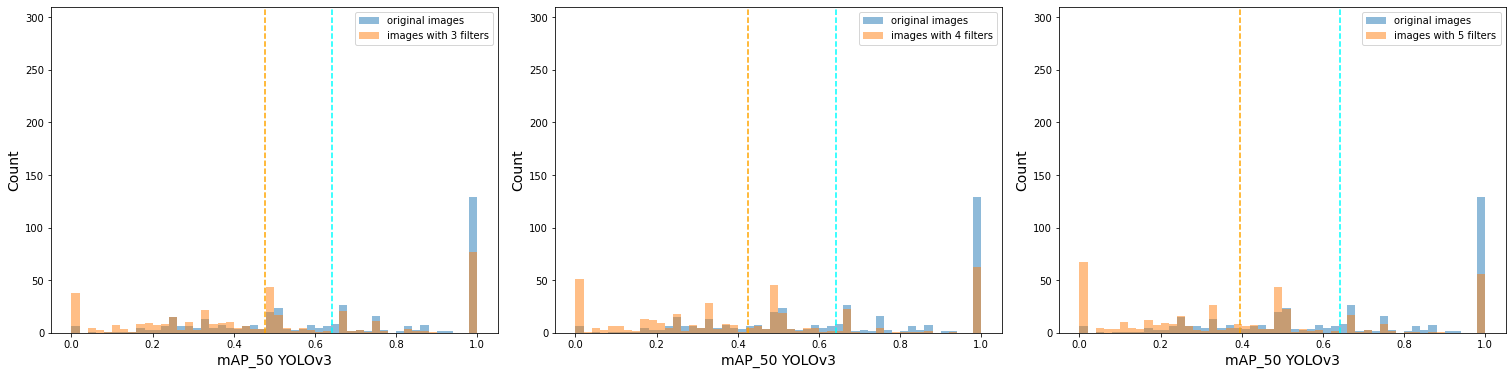
\includegraphics[width=1\textwidth]{Experiments/imgs/y3.png}
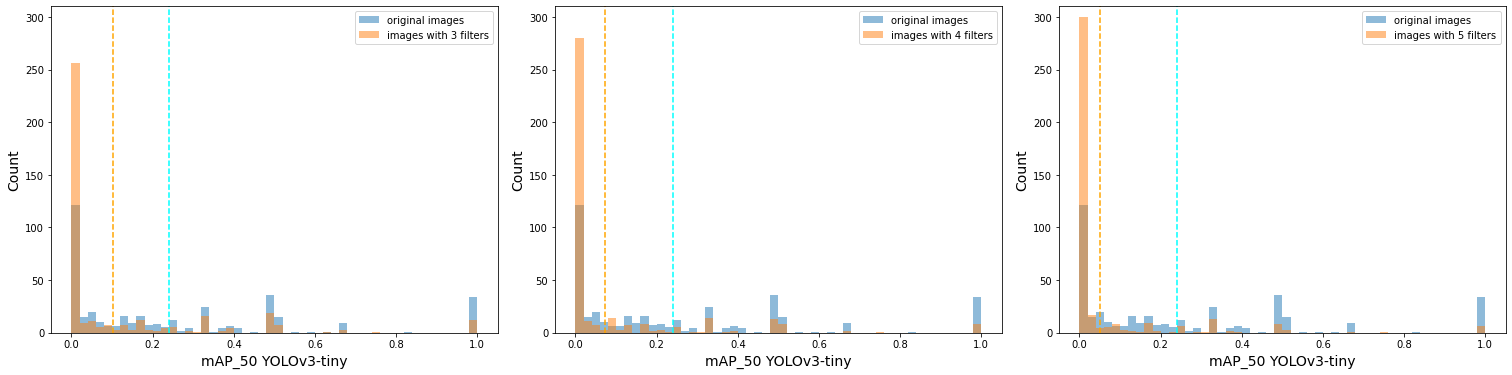
\includegraphics[width=1\textwidth]{Experiments/imgs/y3t.png}
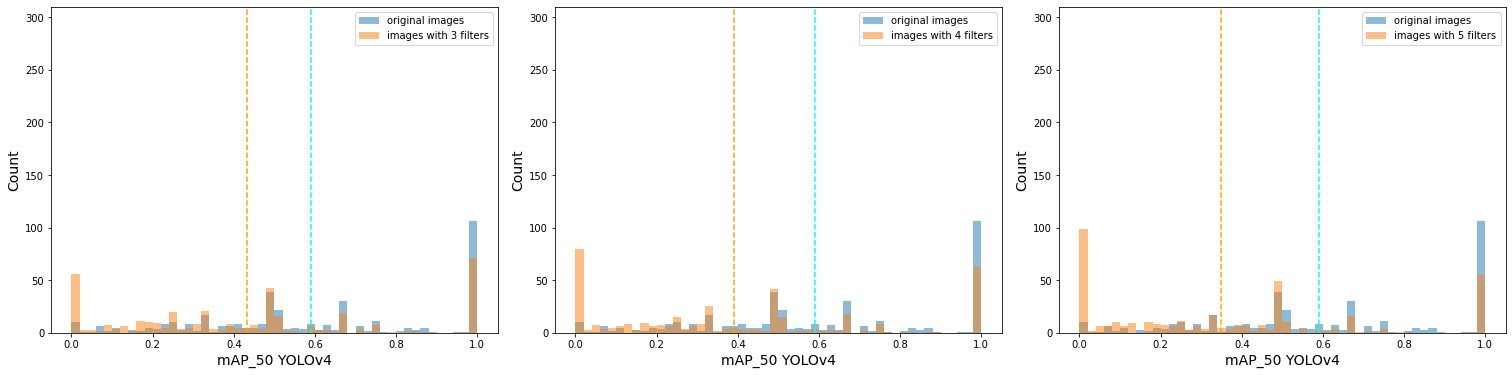
\includegraphics[width=1\textwidth]{Experiments/imgs/y4.png}
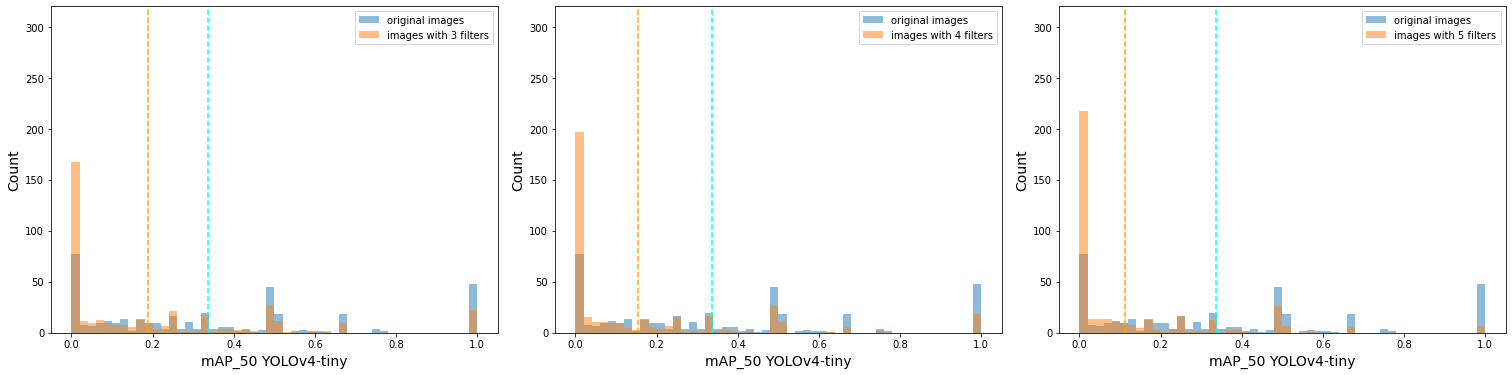
\includegraphics[width=1\textwidth]{Experiments/imgs/y4t.png}
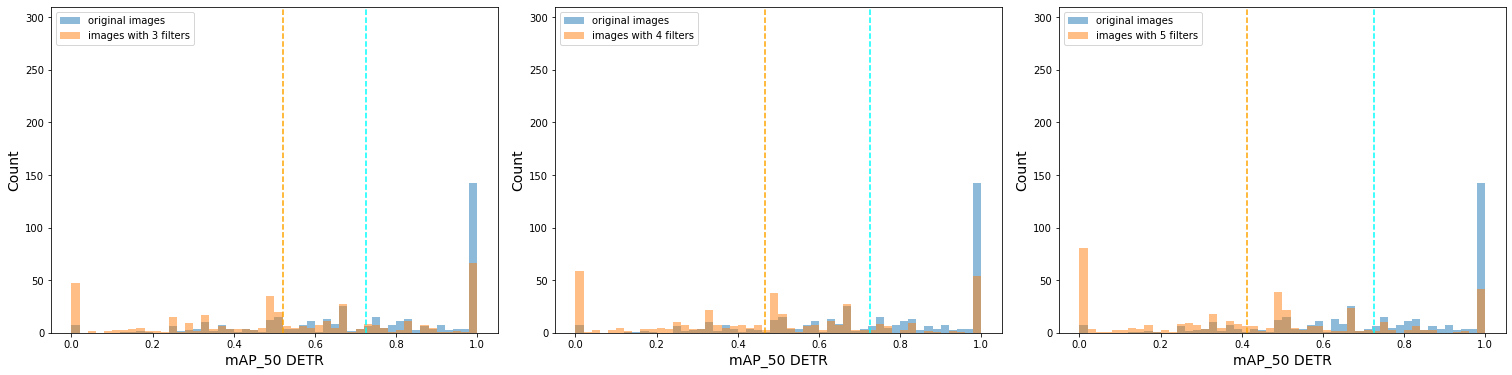
\includegraphics[width=1\textwidth]{Experiments/imgs/detr.png}
\caption{Distribution of AP\_50 values obtained on YOLOv3, YOLOv3-tiny, YOLOv4, YOLOv4-tiny, DETR. The vertical blue dotted line represents the mean over all the mAP\_50 values of the original images. The orange one represents the mean over all the mAP\_50 values of the filtered images}
\label{hysto_objDet}
\end{figure}


If we observe the number of images where all the objects disappear (mAP\_50=0 can be effectively taken as an additional measure for the model robustness) as we espect, besides the mAP\_50 value on 3 filters, YOLOv4 confirms to be the most robustness model and as we expected, both the tiny versions present an impressive robustness decrease with respect their original version. 

An unexpected result can be seen on the decrease of the mAP value in DETR, despite being the best performing model on the clean dataset, the combination of 5 filters decreased its mAP by 53\%.

This behaviour can be observed also analyzing the Precision values in Table \ref{tab_objDet}.


\begin{table}[H]\caption{YOLO and DETR Attack results. Precision and Recall values are calculated with IOU threshold 0.5.\\
In BRISQUE, the lower the score, the better the image quality should be (↓). \\In NIMA, the higher the score, the better the image quality should be (↑).}
\centering
\resizebox{\textwidth}{!}{%
\label{tab_objDet}
\begin{tabular}{llllllllll}
\hline
\multicolumn{10}{c}{\textbf{YOLOv3}} \\ \hline
 & mAP & mAP\_50 & mAP\_75 & precision & recall & SSIM↑ & NIMA↑ & BRISQUE↓ &  \\ \cline{2-9}
no filters & 0.32 & 0.51 & 0.35 & 0.53 & 0.53 & 1.00 & 5.07 & 51.49 &  \\
3 filters & 0.22 (-30\%) & 0.35 & 0.25 & 0.24 & 0.35 & 0.86 & 4.77 & 56.18 &  \\
4 filters & 0.21 (-36\%) & 0.32 & 0.23 & 0.21 & 0.32 & 0.83 & 4.76 & 57.08 &  \\
5 filters & 0.19 (-42\%) & 0.30 & 0.20 & 0.19 & 0.30 & 0.79 & 4.75 & 57.56 &  \\ \hline
\end{tabular}
}
\end{table}

\begin{table}[H]
\resizebox{\textwidth}{!}{%
\begin{tabular}{llllllllll}
\hline
\multicolumn{10}{c}{\textbf{YOLOv3-tiny}} \\ \hline
 & mAP & mAP\_50 & mAP\_75 & precision & recall & SSIM↑ & NIMA↑ & BRISQUE↓ &  \\ \cline{2-9}
no filters & 0.10 & 0.18 & 0.11 & 0.07 & 0.18 & 1.00 & 5.07 & 51.49 &  \\
3 filters & 0.04 (-62\%) & 0.07 & 0.04 & 0.01 & 0.07 & 0.86 & 4.78 & 57.84 &  \\
4 filters & 0.03 (-74\%) & 0.04 & 0.03 & 0.00 & 0.04 & 0.81 & 4.77 & 58.27 &  \\
5 filters & 0.02 (-80\%) & 0.03 & 0.02 & 0.00 & 0.03 & 0.79 & 4.76 & 58.17 &  \\ \hline
\end{tabular}%
}
\end{table}

\begin{table}[H]
\resizebox{\textwidth}{!}{%
\begin{tabular}{llllllllll}
\hline
\multicolumn{10}{c}{\textbf{YOLOv4}} \\ \hline
 & mAP & mAP\_50 & mAP\_75 & precision & recall & SSIM↑ & NIMA↑ & BRISQUE↓ &  \\ \cline{2-9}
no filters & 0.34 & 0.47 & 0.38 & 0.47 & 0.49 & 1.00 & 5.07 & 51.49 &  \\
3 filters & 0.23 (-32\%) & 0.31 & 0.26 & 0.23 & 0.32 & 0.87 & 4.78 & 57.45 &  \\
4 filters & 0.21 (-39\%) & 0.29 & 0.23 & 0.20 & 0.29 & 0.82 & 4.77 & 57.68 &  \\
5 filters & 0.18 (-47\%) & 0.24 & 0.20 & 0.12 & 0.26 & 0.78 & 4.75 & 58.18 &  \\ \hline
\end{tabular}%
}
\end{table}



\begin{table}[H]
\resizebox{\textwidth}{!}{%
\begin{tabular}{llllllllll}
\hline
\multicolumn{10}{c}{\textbf{YOLOv4-tiny}} \\ \hline
 & mAP & mAP\_50 & mAP\_75 & precision & recall & SSIM↑ & NIMA↑ & BRISQUE↓ &  \\ \cline{2-9}
no filters & 0.15 & 0.24 & 0.17 & 0.16 & 0.25 & 1.00 & 5.07 & 51.49 &  \\
3 filters & 0.08 (-47\%) & 0.12 & 0.09 & 0.04 & 0.13 & 0.86 & 4.77 & 57.03 &  \\
4 filters & 0.06 (-57\%) & 0.06 & 0.07 & 0.01 & 0.10 & 0.81 & 4.77 & 56.98 &  \\
5 filters & 0.05 (-66\%) & 0.08 & 0.06 & 0.01 & 0.08 & 0.77 & 4.75 & 57.66 &  \\ \hline
\end{tabular}%
}
\end{table}

\begin{table}[H]
\resizebox{\textwidth}{!}{%
\begin{tabular}{llllllllll}
\hline
\multicolumn{10}{c}{\textbf{DETR}} \\ \hline
 & mAP & mAP\_50 & mAP\_75 & precision & recall & SSIM↑ & NIMA↑ & BRISQUE↓ &  \\ \cline{2-9}
no filters & 0.44 & 0.63 & 0.46 & 0.72 & 0.70 & 1.00 & 5.07 & 51.49 &  \\
3 filters & 0.29 (-33\%) & 0.41 & 0.30 & 0.38 & 0.46 & 0.85 & 4.77 & 57.28 &  \\
4 filters & 0.26 (-40\%) & 0.38 & 0.27 & 0.32 & 0.42 & 0.82 & 4.76 & 57.51 &  \\
5 filters & 0.21 (-53\%) & 0.31 & 0.21 & 0.24 & 0.36 & 0.78 & 4.74 & 57.67 &  \\ \hline
\end{tabular}%
}
\end{table}
In Table \ref{tab_objDet} also the average values for SSIM, NIMA and BRISQUE are provided. \\ \\
\noindent NIMA and BRISQUE are two no reference indexes for Image quality assessment, unlike SSIM we do not use them to optimize filters, but they can be a useful measure to show the overall quality of the images as we increase the number of filters used.

\begin{description}
\item[NIMA:] it uses a CNN model which can be trained to evaluate the aesthetic quality of an image, giving importance to factors like contrast, tone, composition, framing and color palette \cite{NIMA}.
\item[BRISQUE:] it compares statistics of distorted images with the ones of  natural images. It performs well in distortions like noise, blur and JPEG compression \cite{brisque}.
\end{description}

These tho values in table \ref{tab_objDet} show that overall the adversarial images are natural looking and artifact-free.

In this case, while it is easy to note that SSIM index decreases when filters increase, it is not possible to identify a specific pattern across the networks and we can conclude that, at least for these first experiments, the quality of the images performing the attacks does not depend on the model we are attacking
Anyway, also in the case of attacks with 5 filters the SSIM values reported show that the image quality is very good.

The comparisons with other state-of-the-art method discussed in Section \ref{sec:related} need to take into account different aspects. Some papers, like \cite{procNoise_co2019,Lu_2020_CVPR} used global \textit{mAP}, while others,  like \cite{wang2020adversarial} used metrics different from the standard \textit{mAP}. We chose to use \textit{mAP\_, mAP\_75 and mAP\_50}.
Direct and fair comparisons can be made with PRFA\cite{liang2021parallel} that reaches   $mAP\_50=0.46$ on YOLOv3, a value significantly higher than the $mAP\_50=0.30$ reached by our algorithm. 

An important consideration that has to be made, is that none of the cited methods presented results to evaluate image quality. Neither in terms of full-reference measures like SSIM nor in terms of no-reference measures like NIMA \cite{NIMA}. For example, in \cite{procNoise_co2019} the authors showed very good results in terms of mAP, but the images their algorithm produced do not have a good quality since they show very impacting patterns and highly visible artifacts. In Fig \ref{fig:procnoise_samples} some of the images produced are shown. This behaviour is common to the most of restricted  $L_p$-bounded attacks since $L_p$-norms are able to measure the absolute difference between the original image and the modified one, but they cannot capture in any way the image quality in terms of perception.

Finally we also compared the efficiency of the algorithms in terms of number of queries. 
 All the systems proposed in literature need a huge amount of queries and, also in the case of systems built to work with limited access to the victim model, several thousands of queries are needed to produce reliable attacks : $\simeq 30k$ for \cite{wang2020adversarial}, $4k$ for PRFA \cite{liang2021parallel}.
Our algorithm requires a very low number of queries to find an attack: considering the queries computations introduced in (\ref{eq:queries}) and the parameters setting specified in Section \ref{sec:ExpSetUp_objdet}, the maximum number of allowed queries is 490. 
The drawback of using an (apparently expensive) evolutionary approach is highly mitigated by the needed reduced number of generations and population size.\\

It can be noted that an attack can happen in 2 different occurrences:
The most common one is called object disappearance and it happens when the object is not detected in the first place, an example is shown in Figure \ref{fig:objdet_samples} where a kite is no longer detected by YOLOv3 after applying the optimized filters.
The second one is called misclassification and it happens when the object is detected but it has the wrong label like in Figure \ref{fig:objdet_samples_detr} where the previously detected objects are misclassified as “orange” and “bottle”.\\ \\
\noindent\textbf{Transferability} \\
It is usually unknown which architecture a detector uses.
In such case AGV is more effective if it is transferable among different detectors.
For that we tested the transferability of the attacks performed on DETR to the other YOLO models (table \ref{tab_transfer}).
To do that we used the different combination of filters optimized with AGV on DETR and we tested them on YOLO detectors.
As we can see in Fig \ref{hysto_transfer} there is a noticeable increase of the images where mAP\_50 dropped to 0 (the orange column on 0.0).
This suggests that there is some degree of attack transferability between models.

\begin{figure}[h] 
\centering
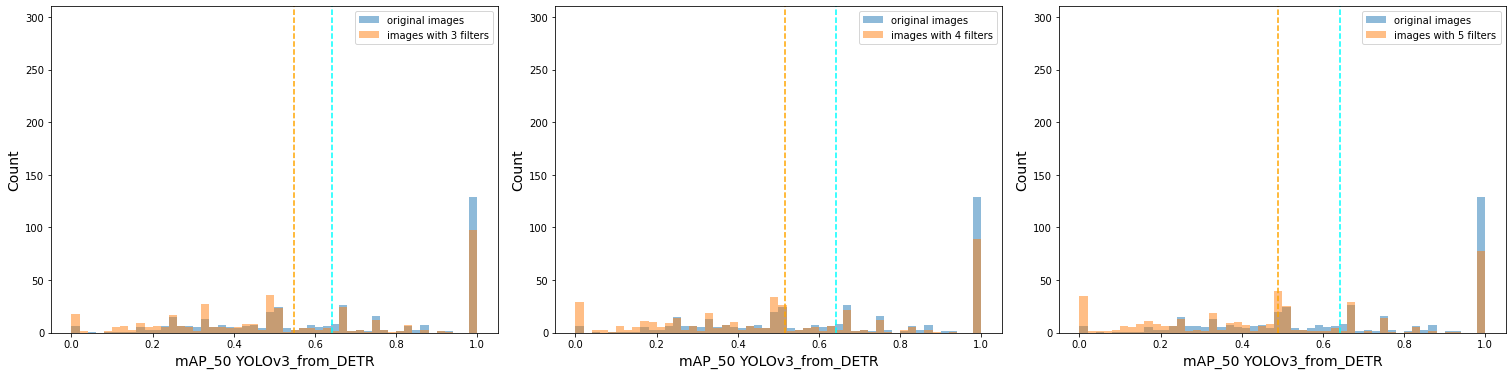
\includegraphics[width=1\textwidth]{Experiments/imgs/y3d.png}
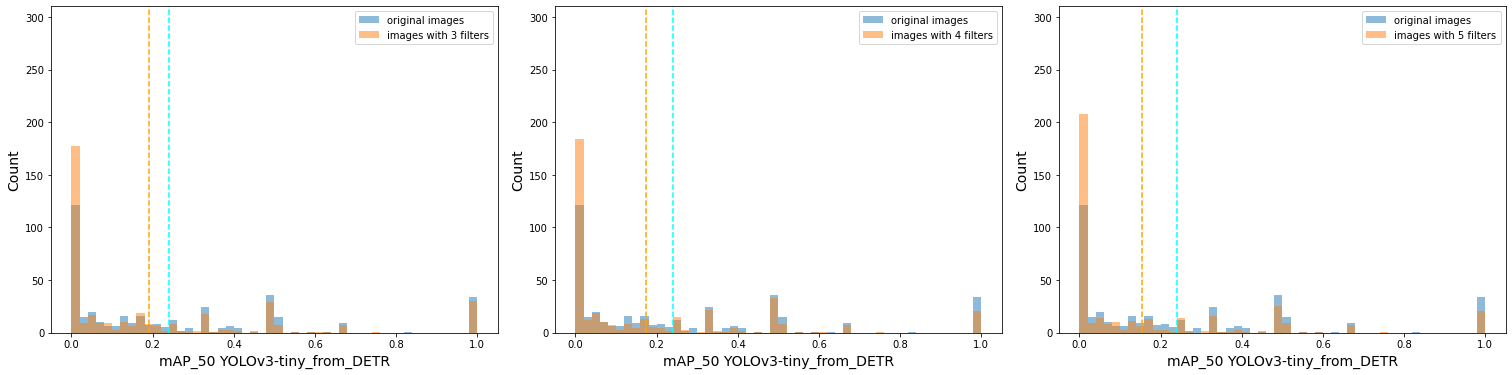
\includegraphics[width=1\textwidth]{Experiments/imgs/y3td.png}
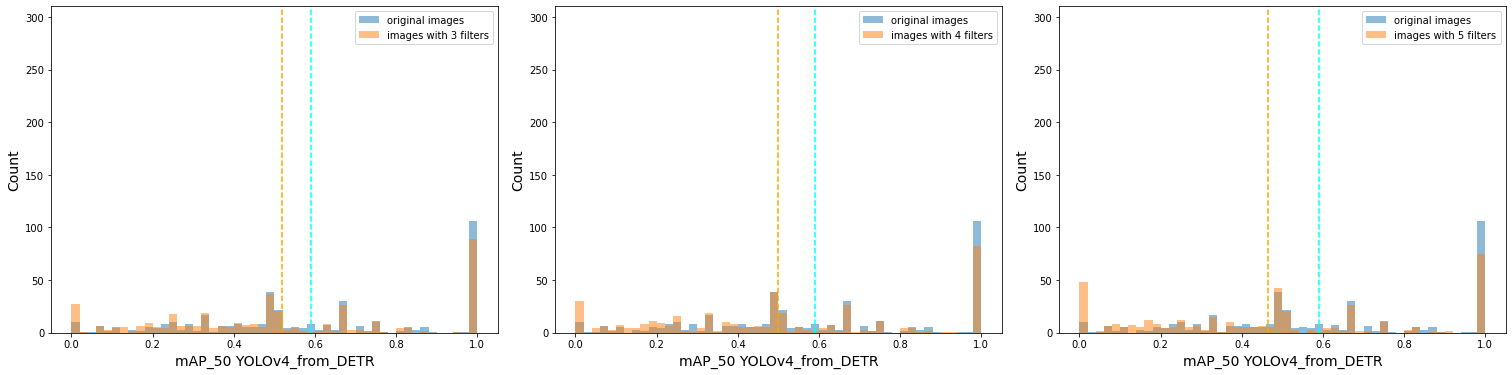
\includegraphics[width=1\textwidth]{Experiments/imgs/y4d.png}
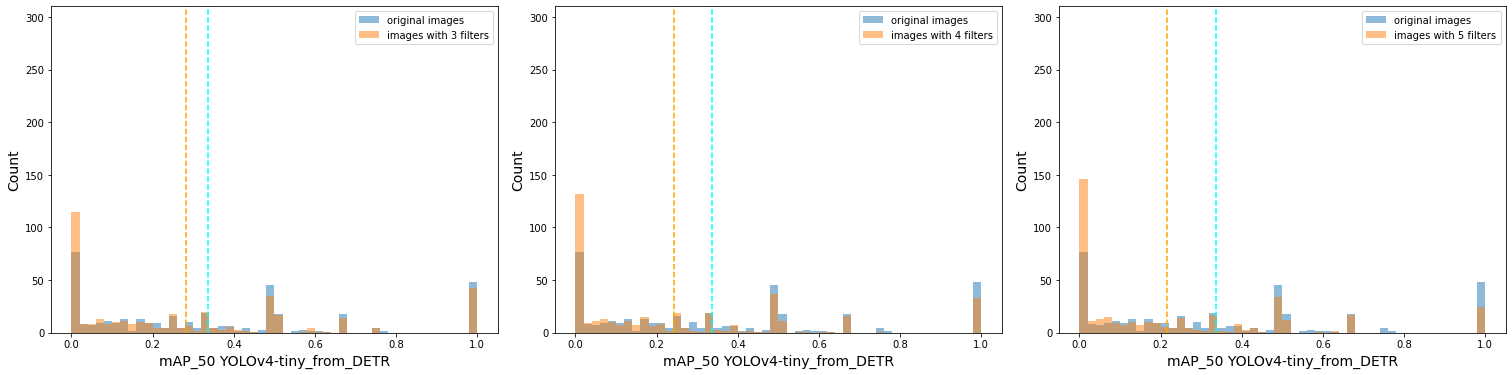
\includegraphics[width=1\textwidth]{Experiments/imgs/y4td.png}
\caption{Distribution of mAP\_50 values obtained on YOLOv3, YOLOv3-tiny, YOLOv4, YOLOv4-tiny from DETR-optimized filters. The vertical blue dotted line represents the mean over all the mAP\_50 values of the original images. The orange one represents the mean over all the mAP\_50 values of the filtered images}
\label{hysto_transfer}
\end{figure}

\begin{table}[H]\caption{YOLO and DETR Attack results. Precision and Recall values are calculated with IOU threshold 0.5.\\
In BRISQUE, the lower the score, the better the image quality should be (↓). \\In NIMA, the higher the score, the better the image quality should be (↑).}
\label{tab_transfer}
\resizebox{\textwidth}{!}{%
\begin{tabular}{llllllllll}
\hline
\multicolumn{10}{c}{\textbf{YOLOv3 (with DETR filters)}} \\ \hline
 & mAP & mAP\_50 & mAP\_75 & precision & recall & SSIM↑ & NIMA↑ & BRISQUE↓ &  \\ \cline{2-9}
no filters & 0.32 & 0.51 & 0.35 & 0.53 & 0.53 & 1.00 & 5.07 & 51.49 &  \\
3 filters & 0.26 (-19\%) & 0.41 & 0.28 & 0.39 & 0.43 & 0.85 & 4.77 & 57.28 &  \\
4 filters & 0.25 (-22\%) & 0.40 & 0.27 & 0.35 & 0.41 & 0.82 & 4.76 & 57.51 &  \\
5 filters & 0.22 (-31\%) & 0.36 & 0.25 & 0.30 & 0.30 & 0.78 & 4.74 & 57.67 &  \\ \hline
\end{tabular}%
}
\end{table}


\begin{table}[H]
\resizebox{\textwidth}{!}{%
\begin{tabular}{llllllllll}
\hline
\multicolumn{10}{c}{\textbf{YOLOv3-tiny (with DETR filters)}} \\ \hline
 & mAP & mAP\_50 & mAP\_75 & precision & recall & SSIM↑ & NIMA↑ & BRISQUE↓ &  \\ \cline{2-9}
no filters & 0.10 & 0.18 & 0.11 & 0.07 & 0.18 & 1.00 & 5.07 & 51.49 &  \\
3 filters & 0.08 (-27\%) & 0.13 & 0.07 & 0.03 & 0.13 & 0.85 & 4.77 & 57.28 &  \\
4 filters & 0.07 (-32\%) & 0.12 & 0.08 & 0.03 & 0.12 & 0.82 & 4.76 & 57.51 &  \\
5 filters & 0.06 (-39\%) & 0.11 & 0.07 & 0.03 & 0.11 & 0.78 & 4.74 & 57.67 &  \\ \hline
\end{tabular}%
}
\end{table}

\begin{table}[H]
\resizebox{\textwidth}{!}{%
\begin{tabular}{llllllllll}
\hline
\multicolumn{10}{c}{\textbf{YOLOv4 (with DETR filters)}} \\ \hline
 & mAP & mAP\_50 & mAP\_75 & precision & recall & SSIM↑ & NIMA↑ & BRISQUE↓ &  \\ \cline{2-9}
no filters & 0.34 & 0.47 & 0.38 & 0.47 & 0.49 & 1.00 & 5.07 & 51.49 &  \\
3 filters & 0.29 (-13\%) & 0.41 & 0.32 & 0.39 & 0.43 & 0.85 & 4.77 & 57.28 &  \\
4 filters & 0.28 (-18\%) & 0.38 & 0.31 & 0.30 & 0.40 & 0.82 & 4.76 & 57.51 &  \\
5 filters & 0.24 (-27\%) & 0.34 & 0.28 & 0.25 & 0.36 & 0.78 & 4.74 & 57.67 &  \\ \hline
\end{tabular}%
}
\end{table}

\begin{table}[H]
\resizebox{\textwidth}{!}{%
\begin{tabular}{llllllllll}
\hline
\multicolumn{10}{c}{\textbf{YOLOv4-tiny (with DETR filters)}} \\ \hline
 & mAP & mAP\_50 & mAP\_75 & precision & recall & SSIM↑ & NIMA↑ & BRISQUE↓ &  \\ \cline{2-9}
no filters & 0.15 & 0.24 & 0.17 & 0.16 & 0.25 & 1.00 & 5.07 & 51.49 &  \\
3 filters & 0.11 (-23\%) & 0.19 & 0.13 & 0.08 & 0.19 & 0.85 & 4.77 & 57.28 &  \\
4 filters & 0.10 (-32\%) & 0.16 & 0.11 & 0.05 & 0.16 & 0.82 & 4.76 & 57.51 &  \\
5 filters & 0.09 (-42\%) & 0.14 & 0.09 & 0.04 & 0.14 & 0.78 & 4.74 & 57.67 &  \\ \hline
\end{tabular}%
}
\end{table}

\begin{figure}[h]% 
    \centering
    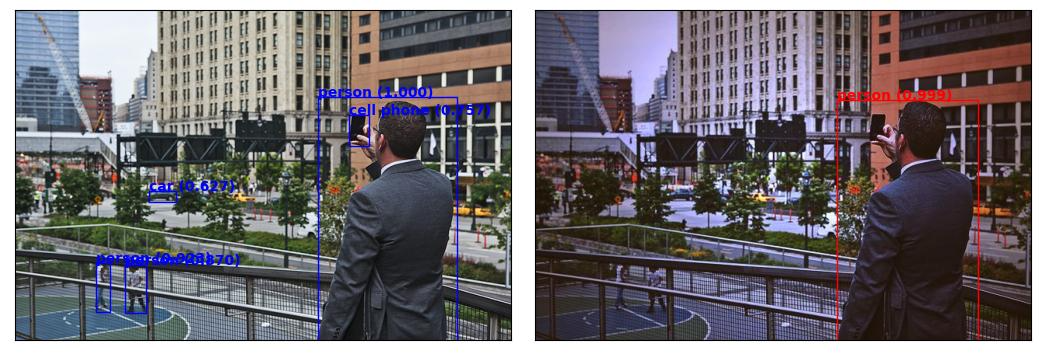
\includegraphics[width=0.85\textwidth]{Experiments/imgs/0.8_545100.png}
    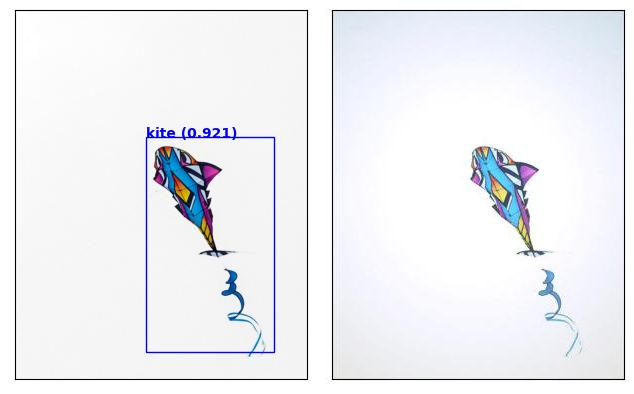
\includegraphics[width=0.85\textwidth]{Experiments/imgs/1_85665.png}
    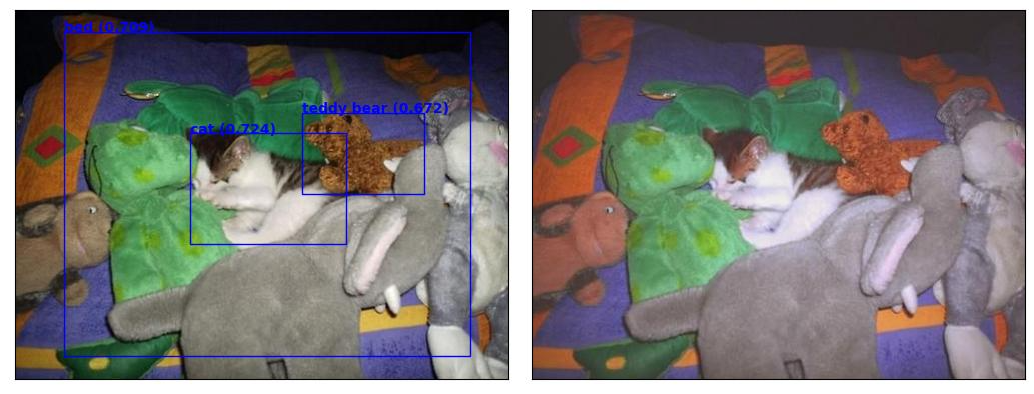
\includegraphics[width=0.85\textwidth]{Experiments/imgs/1_434996.png}
    \caption{On the left: images without filters and YOLOv3 detected bounding-boxes (in blue). On the right: images with 4 adversarial filters and YOLOv3 detected bounding-boxes (in red).}
    \label{fig:objdet_samples}
\end{figure}

\begin{figure}[h]% 
    \centering
    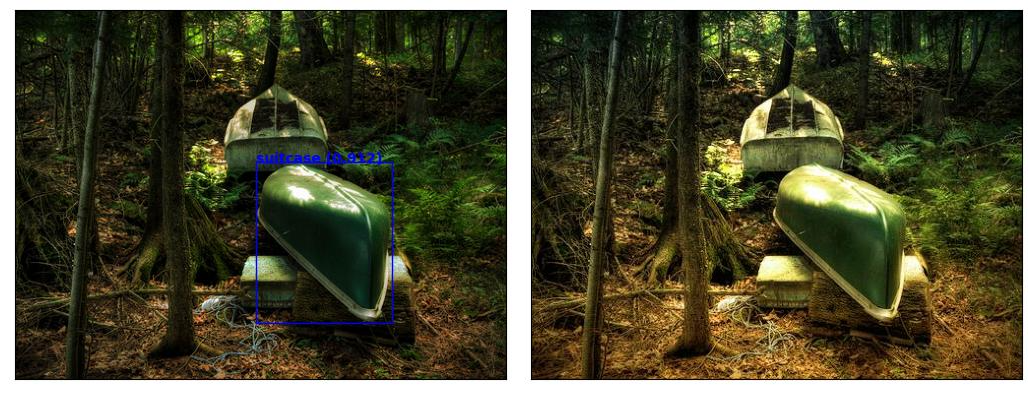
\includegraphics[width=0.85\textwidth]{Experiments/imgs/imgdetr1.png}
    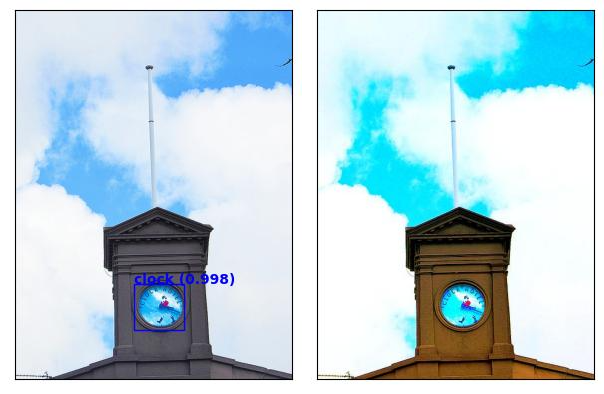
\includegraphics[width=0.85\textwidth]{Experiments/imgs/imgdetr2.png}
    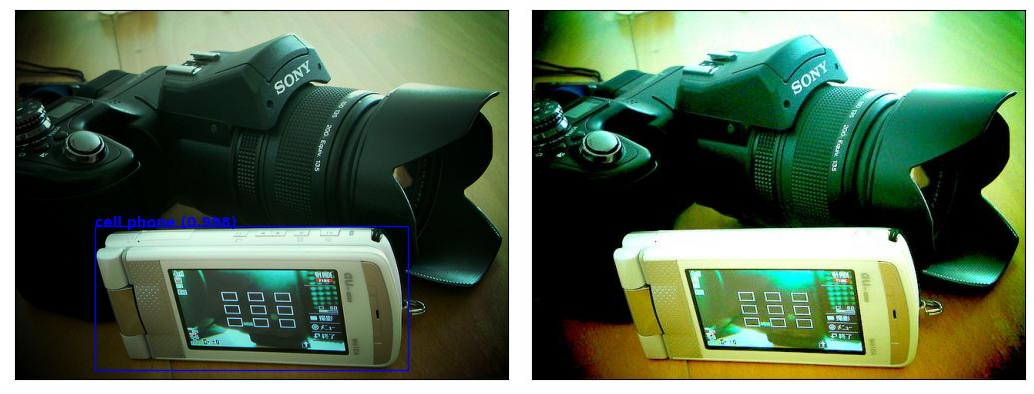
\includegraphics[width=0.85\textwidth]{Experiments/imgs/imgdetr4.png}
    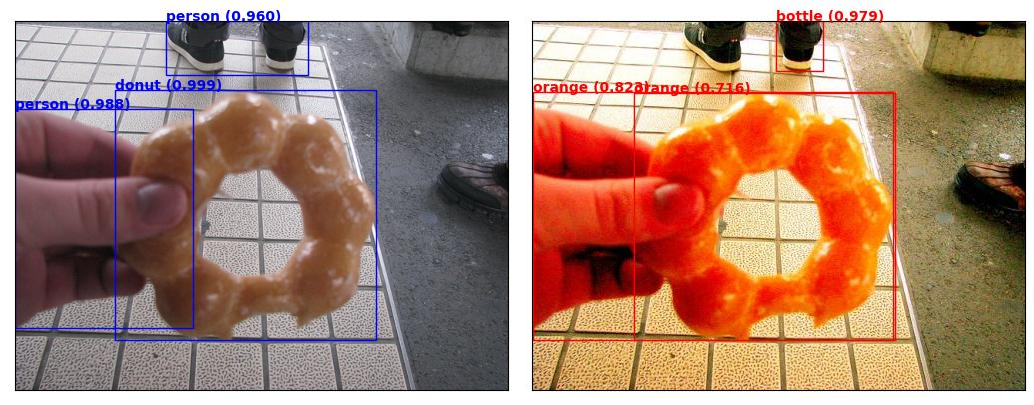
\includegraphics[width=0.85\textwidth]{Experiments/imgs/imgdetr5.png}
    \caption{On the left: images without filters and DETR detected bounding-boxes (in blue). On the right: images with 3 adversarial filters and DETR detected bounding-boxes (in red).}
    \label{fig:objdet_samples_detr}
\end{figure}

\begin{figure}[h]
    \centering
    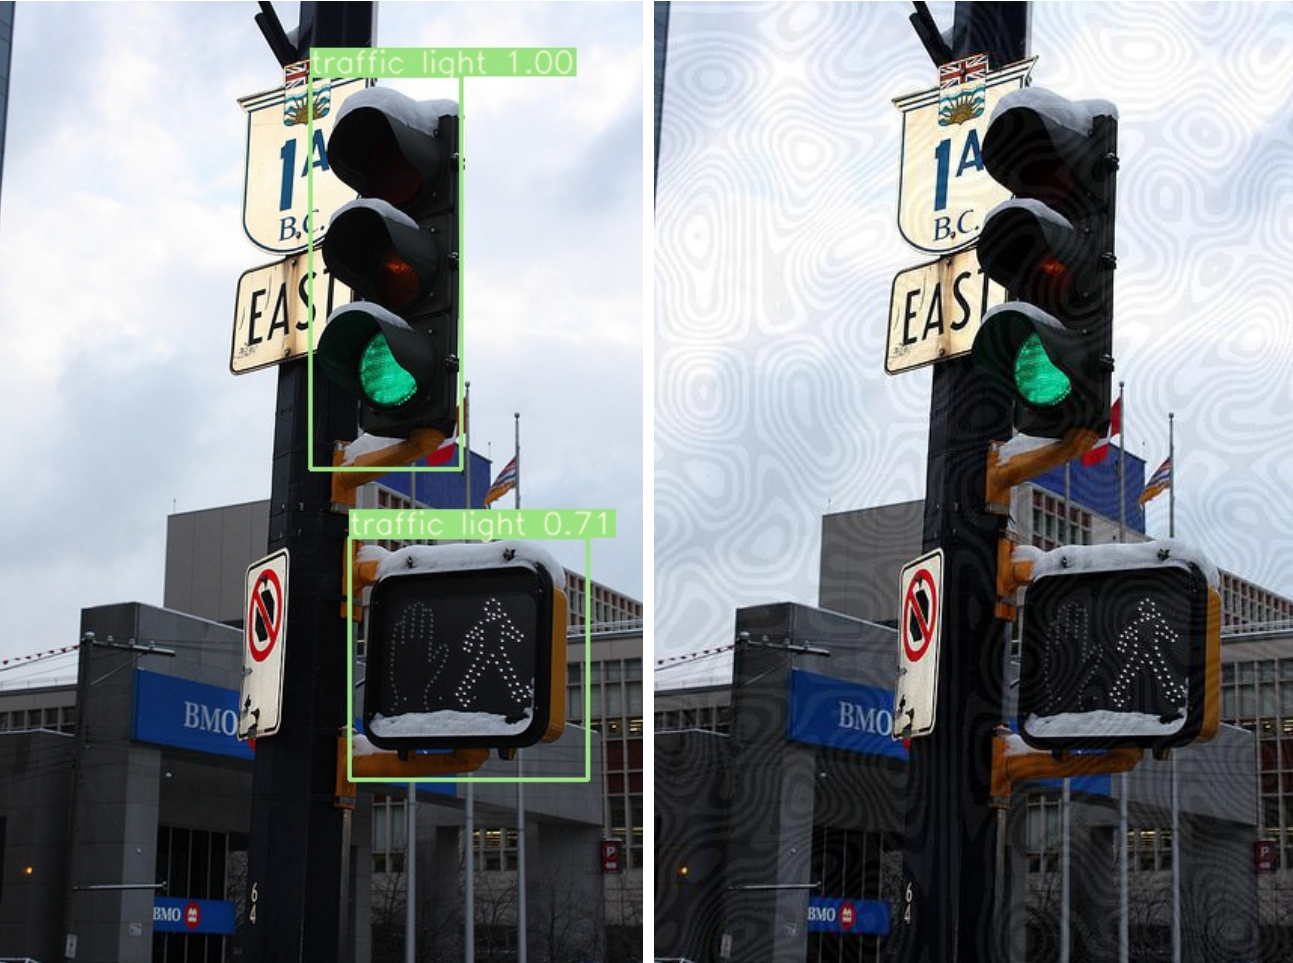
\includegraphics[width=0.8\textwidth]{Experiments/imgs/semaforo.png}
    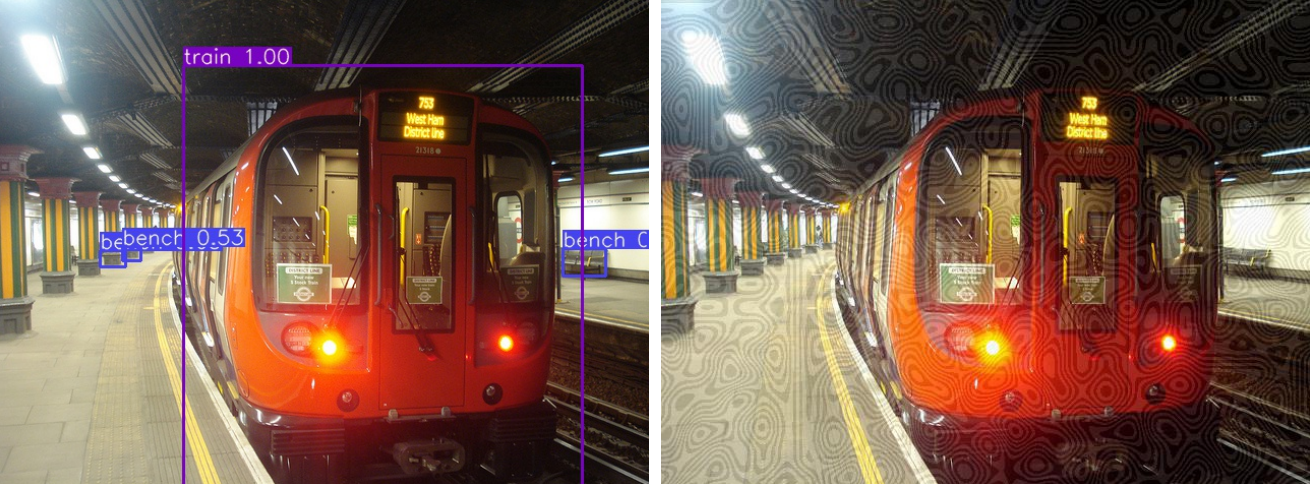
\includegraphics[width=0.8\textwidth]{Experiments/imgs/treno.png}
    \caption{Perlin noise adversarial examples on YOLO v3 from \cite{procNoise_co2019}}
    \label{fig:procnoise_samples}
\end{figure}



